
%place your content here, feel free to create subcontent files

\begin{block}{\blocktitle{Abstract}}
\justifying
We propose minimum regret search (MRS), a novel acquisition function for Bayesian
optimization. MRS bears similarities with information-theoretic approaches
such as entropy search (ES). However, while ES aims in each query at maximizing the
information gain with respect to the global maximum, MRS aims at minimizing the
expected simple regret of its ultimate recommendation for the optimum. While empirically ES and MRS perform similar in most of the
cases, MRS produces fewer outliers with high simple regret than ES. We provide empirical
results both for a synthetic single-task optimization problem as well as for a
simulated multi-task robotic control problem.
\end{block}

\begin{block}{\blocktitle{Background}}
\textbf{Contextual policy search} \cite{deisenroth_survey_2013} aims at learning an upper-level policy $\pi_\omega(\theta \vert s)$, where
\begin{itemize}
 \item $s \in \mathbb{R}^{n_s}$ encodes the current context (task)
 \item $\theta \in \mathbb{R}^{n_\theta}$ is a parameter vector for a lower-level policy such as a DMP \cite{ijspeert_dynamical_2013}
 \item $\omega \in \mathbb{R}^{n_\omega}$ is the parameter vector of the upper-level policy to be learned
\end{itemize}
such that the expected return over all contexts $J_\omega = \int_s \mu(s) \int_\theta \pi_\omega(\theta \vert s) R(s, \theta) ds d\theta$ is maximized.

One class of contextual policy search methods are \textbf{gradient-free, local-search methods} such as cost-regularized kernel regression \cite{Kober2012} and contextual relative entropy search (C-REPS) \cite{kupcsik_data-efficient_2013}.

\textbf{Bayesian optimization for contextual policy search (BO-CPS)} \cite{metzen_bayesian_2015} is an alternative model-based global-search approach, which is very efficient for low-dimensional search spaces combined with an expensive cost function.
\begin{itemize}
 \item Use surrogate model (Gaussian process) to model expected return for context-parameter pairs (allows generalization over similar contexts)
 \item Acquisition function: GP upper confidence bound (GP-UCB) \cite{srinivas_gaussian_2010}, entropy search \cite{hennig_entropy_2012}
 \item Perform optimization (DIRECT + L-BFGS) of acquisition function over parameter space for fixed context (context determined by the environment or chosen randomly)
\end{itemize}

\end{block}

\begin{block}{\blocktitle{Active Contextual Entropy Search}}
\emph{Idea:} Extend entropy search such that it allows selecting \emph{actively} the context for the next trial, in which it expects to learn the most

Entropy Search (ES):
\begin{itemize}
 \item estimate probability $p_{opt}(\theta)$ that the global optimum of unknown function $f$ is at $\theta$ at finitely many points $\{\theta^c\}_{i=1}^{N_\theta}$ and approximate using Monte Carlo integration
 \item predict the change of GP when drawing a sample at the query point
$\theta^q$ and assuming $N_y$ different outcomes $\{y^{(i)}\}$ sampled from the
GP's predictive distribution at $\theta^q$
 \item select query point that minimizes the average loss (maximizes the relative entropy) $\mathcal{L}(p_{opt}[\theta^q]) = - \int p_{opt}[\theta^q](\theta) \log \frac{p_{opt}[\theta^q](\theta)}{U_I(\theta)}, \text{d}\theta$,  where $p_{opt}[\theta^q]$ denotes the probability
 distribution of the global optimum \emph{after} an assumed query at $\theta^q$.
\end{itemize}

Active Contextual Entropy Search (ACES):
\begin{itemize}
 \item Let $p_{max}(\theta \vert s)$ denote the CPD that maximum return given context $s$ is at $\theta$
 \item Loss: expected change of relative entropy in context $s$ after performing a trial in context $s^q$with parameter $\theta^q$: $\mathcal{L}^s(s^q, \theta^q) = \mathcal{L}(p_{max}[s^q,\theta^q](\theta \vert s)) - \mathcal{L}(p_{max}(\theta \vert s))$
 \item $s^q, \theta^q = \arg\min_{(s^q, \theta^q)} \mathcal{L}^{s^q}(s^q,
\theta^q)$ would not account for information gained about the
optima in contexts $s \neq s^q$
 \item Acquisition function: $\text{ACES}(s^q, \theta^q) = \sum_{i=1}^{N_s}
\mathcal{L}^{s^c_i}(s^q, \theta^q)$, trial contexts $s^c_i \sim \mathcal{U}(S)$
 \item Evaluating $\text{ACES}(s^q, \theta^q)$ is expensive but GP has intrinsic length scales; \\approximate $\text{ACES}(s^q, \theta^q) \approx \sum_{s \in \text{NN}(s^q,
\{s^c\}, N_{nn})}  \mathcal{L}^s(s^q, \theta^q)$
 \item NN returns the $N_{nn}$ nearest neighbors of  $s^q$ in $\{s^c\}$ according to a Mahalanobis distance with the (anisotropic) GP length scales on the diagonal of the covariance
 \item Small $N_{nn}$ is faster but approximates $\text{ACES}(s^q, \theta^q)$ using only local information (local in context space), we compare $N_{nn}=1$ and $N_{nn}=20$
 \item Optimization based on CMA-ES (noisy acquisition function)
\end{itemize}
\end{block}

\begin{block}{\blocktitle{Illustration}}
\vspace*{1cm}

\begin{figure}
\centering
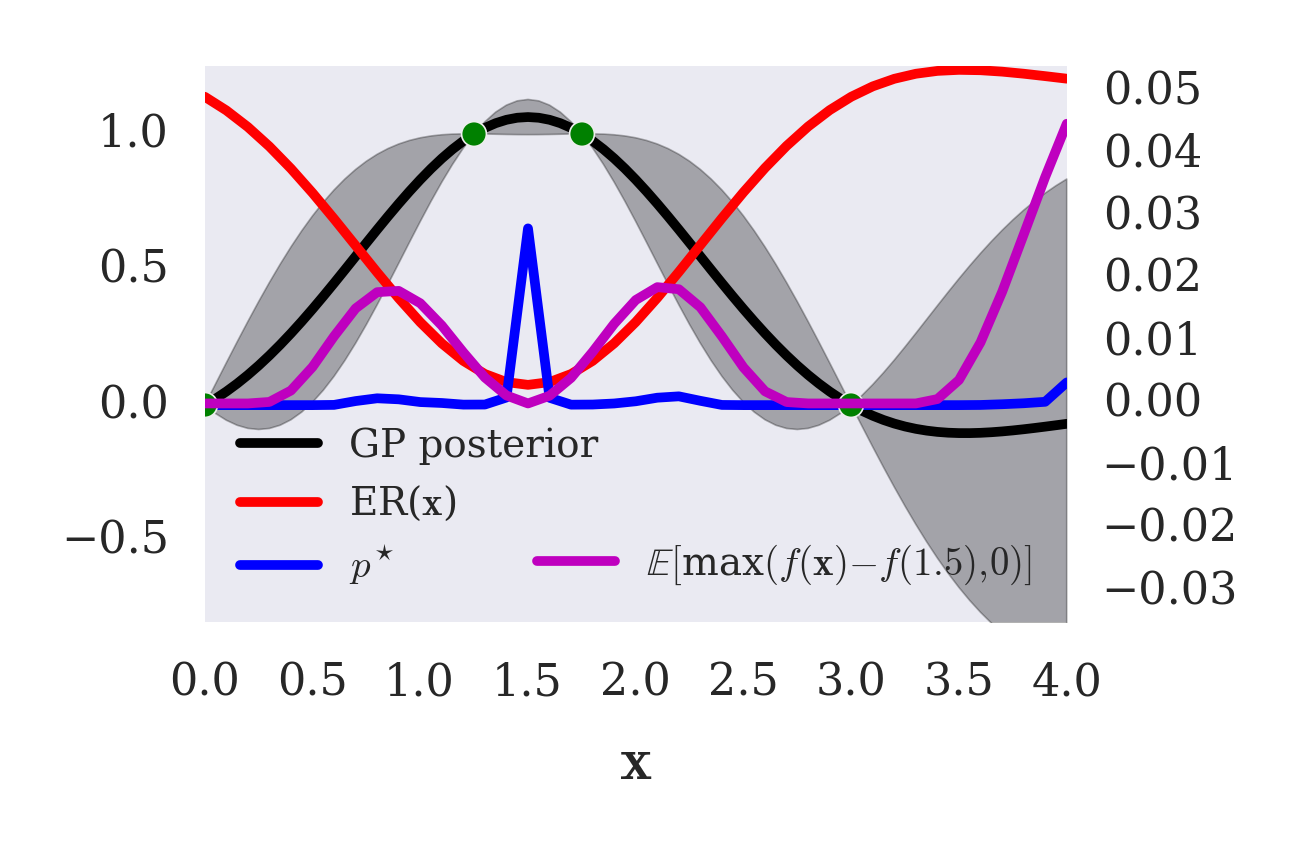
\includegraphics[width=0.4\columnwidth]{../pics/regret_illustration}
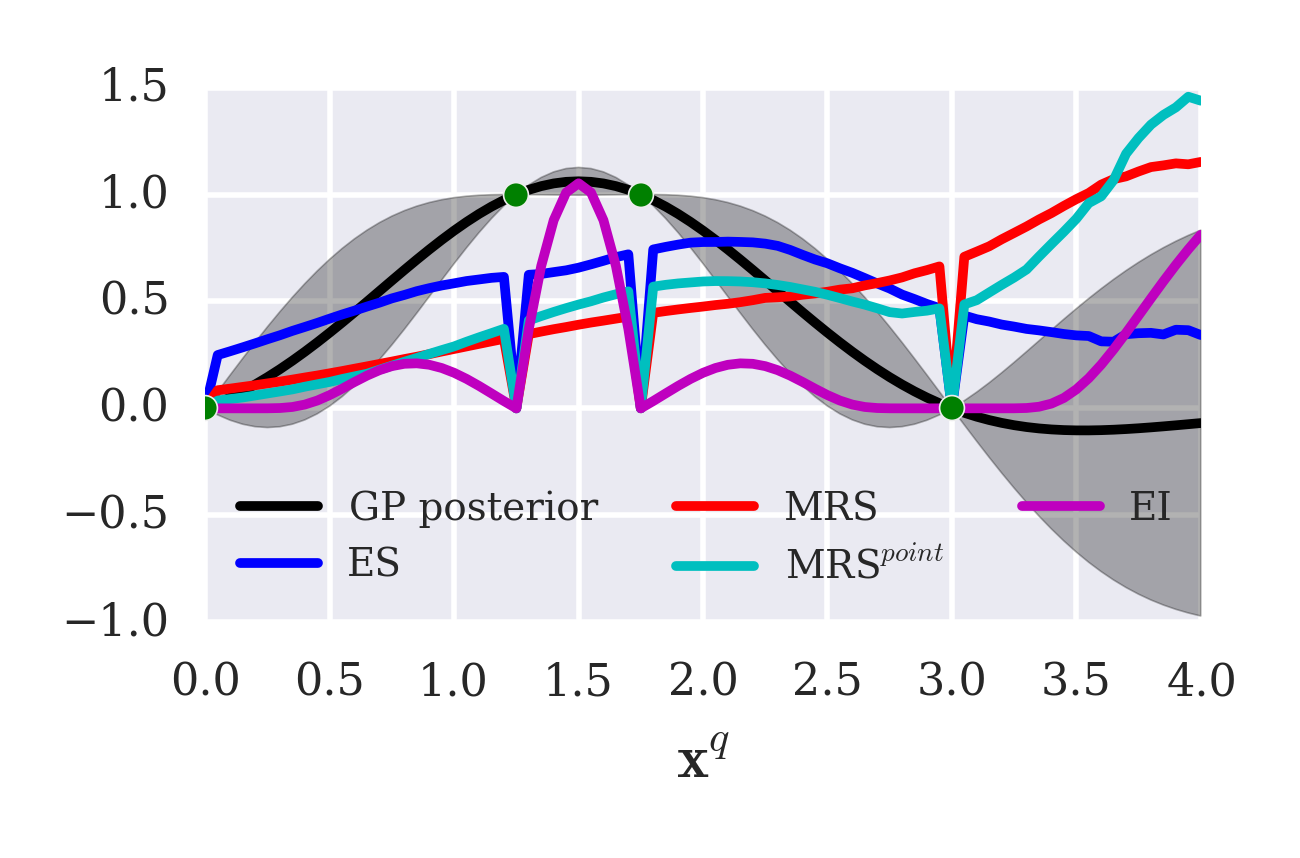
\includegraphics[width=0.4\columnwidth]{../pics/acq_comparison}
\caption{(Left) Illustration of GP posterior, probability of maximum $p^\star$, expected regret ER, and  $\mathbb{E}[\max(f(\mathbf{x}) - f(1.5), 0)]$ (scale on the right-hand side). (Right) Illustration of GP posterior and different acquisition function. Absolute values have been normalized such that the mean value of an acquisition function is $0.5$. Best seen in color.}
\label{fig:MRS_illustration}
\end{figure}

\end{block}